\documentclass[a4paper]{report}
\usepackage{verbatim}
\usepackage{graphicx}
\usepackage{tabularx}
\usepackage{amsfonts}

\title{Thesis}
\author{Ken Williams}
\begin{document}

\maketitle

\chapter*{Abstract}
\chapter*{Acknowledgements}

\tableofcontents

\chapter{Introduction}

\section{Preface}

The field of Automatic Text Categorization is an extremely active area
of current research and application.  It is a multi-disciplinary
field, attracting attention from the Linguistics, Computer Science,
Engineering, and Business communities.  Its applicability is broad,
with many potential uses for large businesses as well as individuals.

The goal of Automatic Text Categorization is to produce specialized
algorithms that can process natural-language documents, assigning zero
or more user-defined labels to them based on their content.  More
formally, given a set of labels $L = \{L_1, \ldots, L_k\}$ and a set of
previously unseen documents $D = \{D_1, D_2, \ldots \}$, a categorizer is a
function $C$ that maps from $D$ to the set of all subsets of $L$.  In
practice, many categorizers assign only a single label to each
document, so a categorizer is often a function that maps directly from
$D$ to $L$.  Often an intermediate function is useful for "soft" or 
"rank-based" categorization, mapping from ordered pairs $(D_i, C_j)$ 
to the set of real numbers $\mathbb{R}$ in order to assign a score 
to each category $C_j$ for each document $D_i$.

The standard modern approach to creating new categorizer functions is
to build them using Machine Learning techniques from a set of training
documents.  This is a set of user-provided, pre-labeled documents that
follows a category
distribution similar to the distribution of $D$, and whose contents
provide information about what sorts of documents should be mapped to
what sorts of categories.  Algorithms can then be developed that make
generalizations about the relationship between document content and
document category, encoding these generalizations in the algorithm $C$.

\section{Automatic Text Categorization}

\section{Object Frameworks}

A framework is a large-scale unit of reusable code in object-oriented
software development.  Frameworks were developed in response to
situations requiring fine-grained control over the

\subsection{Guidelines for designing frameworks}
\subsection{Design patterns}


\section{Overview of AI::Categorizer Framework}

AI::Categorizer is a set of Perl modules that implements an
object-oriented framework for text categorization.  It provides
classes for managing documents, categories, machine learners,
categorization hypotheses, and categorization results.

\section{Contributions}

\section{Organization of the Thesis}

\chapter{Practical Issues in Text Categorization}

\section{Usage Scenarios (use cases)}
\subsection{Commercial scenarios}
\subsection{Research scenarios}

\section{General Text Categorization Considerations}
\subsection{Document format}
\label{Document format}

XXX... However, many Text Categorization data sets are quite large.  They may
commonly be larger than the amount of available memory on the machine
processing them.  This has two important implications.  First,
converting the documents to a special format so that the framework can
access them may be impossible or undesirable for reasons of time,
space, and data redundancy.  Second, a mechanism 

unnecessary copies of the data, 

\subsection{Document structure}
\subsection{Tokenizing of data}
\subsection{Linguistic stemming}
\subsection{Feature selection}
\subsection{Vector space modeling}
\subsection{Machine learning algorithm choice}
\subsection{Machine learning configuration}
\subsection{Incremental or on-line learning}
\subsection{Hypothesis behavior}

\section{Machine learning techniques}
\subsection{Naive Bayes}
\subsection{Decision Trees}
\subsection{Support Vector Machines}

\section{Application integration}
\subsection{Client/server applications}
\subsection{Embedded applications}
\subsection{Database cooperation}

\section{Evaluation}
\subsection{Correctness}
Precision, recall, FN2, error, accuracy
\subsection{Usefulness}
ROC curves
\subsection{Scalability}
\subsubsection{Architecture}
\subsubsection{Running time}
\subsubsection{Memory usage}

\section{Related products}

To establish the relevance of AI::Categorizer in the marketplace of
Text Categorization, I will examine three related products.  First I
discuss Weka, a Java product that has been used successfully by many
Text Categorization researchers.  Then I address two businesses that
supply products and services related to Text Categorization,
Autonomy.com and Teragram Corporation.

\subsection{Weka}

Weka is an open-source system for Machine Learning originally
developed at the XXX University of Waikato, New Zealand.  Its primary
audience is the international community of academic machine learning
researchers, most notably those working with Categorization or
Clustering problems that arise from working with text.  Weka has
undergone at least one major code rewrite; at present it is
implemented as a set of related Java classes with documented internal
interfaces, so it may itself be considered a framework.

Weka is used extensively throughout the academic Text Categorization
community, and as such includes support for many cutting-edge
categorization techniques, including advances in Support Vector
Machines, k-Nearest-Neighbor, Naive Bayes, and other categorizers, as
well as several variations of feature selection techniques.  It is
therefore a standard against which the AI::Categorizer framework can
be measured, as well as a resource which can be leveraged in its
construction.

Despite some similar properties, Weka and AI::Categorizer differ in
their goals and in many important implementation decisions.  Whereas
Weka specifically targets the academic research community,
AI::Categorizer aims to support use cases under both
application-building and research-conducting situations.
Consequently, Weka will typically keep up with research trends more
closely, but AI::Categorizer will usually be easier for application
developers to integrate into a real-world situation.

In addition to these differences, another important difference arises
from the different goals in the two projects.  Much of the academic
community is interested in evaluating the correctness and algorithmic
complexity of categorization techniques, whereas most application
developers must also consider resource usage in real-world terms like
time and memory.  In testing, AI::Categorizer has greatly outperformed
Weka in terms of speed and memory when equivalent algorithms are
compared on identical data sets.  This doesn't reflect an inherent
design flaw in Weka, rather a difference in the kinds of things Weka
developers are likely to spend their time working on.

In order to help facilitate cooperation between the Weka and
AI::Categorizer communities, as well as leverage existing solutions
inside AI::Categorizer, a machine learner class has been created
within AI::Categorizer that simply passes data through to Weka's
categorizers.  In this way, application developers can easily
experiment with Weka's cutting-edge categorization techniques while
retaining AI::Categorizer's application integration advantages.  Any
cross-pollination generated as a result will likely benefit both
projects.

Other facilities provided by Weka are not yet offered by
AI::Categorizer.  These include visualization tools, several
sophisticated correctness evaluation tools, and XXX.  Most of these
facilities would make useful additions to AI::Categorizer if
implemented

\subsection{Autonomy.com}

\subsection{Teragram Corporation}

According to their web site (http://www.teragram.com/), Teragram
Corporation is a provider of ``fast and stable linguistic
technologies, information search and extraction, knowledge management,
and text processing technologies.''  One of their largest-scale
products is the Teragram Categorizer, an automatic document
categorizer that plays a similar technical role to AI::Categorizer.
It cooperates with the Teragram Taxonomy Manager, which provides a
user interface to categories and the documents within each category.

All of Teragram's software products are proprietary, so little
information on implementation is available.  However, product
capabilities and roles can be assessed from the marketing information
given on the web site.  The information presented here has all been
gathered this way.

The Taxonomy Manager is a browser of hierarchical categories, similar
to several on-line directory services like Yahoo
(http://www.yahoo.com/) or the Open Directory Project
(http://www.dmoz.org/).  It might therefore be inferred that the
Categorizer is a native hierarchical categorizer, or perhaps that the
categorizer actually flattens the tree structure of the category
hierarchy into a flat list of its leaves, and imposes the tree
structure only afterwards.  Whichever case is true, it must be noted
that the interfaces of the categorizer allow hierarchical
categorization even if the internal workings are flat.

Another interesting aspect of Teragram's categorization technology is
their Rule-Based Categorizer.  Using this system, ``each category
within the directory is associated with a set of rules that describe
documents within that category.''  This may be motivated by a need to
integrate older hand-maintained lists of rules into newer
applications, or it might be meant to address situations like email
categorization in which most documents are indeed best categorized by
simple rules (usually because the sender and receiver have agreed upon
a tagging scheme to mark documents' important properties).  It's not
clear whether Teragram's Rule-Based Categorizer and Automatic
Categorizer can cooperate on a single taxonomy, but they indicate that
the two systems are complementary rather than antithetic.

Teragram also offers separate licensing for many of the tools that
make up its products.  In this sense, it has a strategy similar to one
employed in AI::Categorizer's design, in which useful pieces of
functionality created for AI::Categorizer should be split off into
their own products whenever possible.

\section{Dissemination}
\subsection{Documentation}
\subsection{Community involvement}

\chapter{AI::Categorizer Framework Design}

The AI::Categorizer framework is designed for maximum re-use in many
kinds of situations \ldots XXX.

For brevity, the ``AI::Categorizer::'' prefix will be omitted from class
names in this discussion.  It is to be understood that any class
within the AI::Categorizer framework (except the top-level class
AI::Categorizer itself) is prefixed by the ``AI::Categorizer::''
namespace.

\section{Overview of AI::Categorizer class hierarchy}

In order to understand the structure of the AI::Categorizer framework,
multiple kinds of analysis are helpful.  We can examine the
inheritance relationships of the classes that participate in
AI::Categorizer, and indicate which classes inherit from each other.
Since a class generally is a representation of certain
responsibilities and capabilities, this lets us see how the set of
responsibilities for one class may be implemented in different ways or
extended by its subclasses.

\begin{figure}
\includegraphics[width=\linewidth]{figures/inheritance-uml.pdf}
\caption{Inheritance diagram for AI::Categorizer}
\label{inheritance-uml}
\end{figure}

Figure \ref{inheritance-uml} shows the inheritance relationships among
classes in the AI::Categorizer framework.  Note that this diagram
indicates the \emph{capabilities} of the framework more than it
indicates its \emph{architecture}.  For instance, the framework
currently understands several document types, including plain text
documents and documents in the ``SMART'' format.  If the framework is
extended by writing additional subclasses of existing classes, the
capabilities increase without changing the basic architecture of the
framework.

Note that the inheritance diagram is not particularly enlightening
about how various classes cooperate to perform text categorization
tasks.  The inheritance relationships are set at compile-time and do
not change while the framework is in use.\footnote{Perl allows the
dynamic reassignment of inheritance, but this capability isn't used
in the framework.}

Another way to examine the framework is to examine the run-time
relationships between its classes.  This often provides a much more
enlightening analysis of a framework, since modern framework design
often favors object composition over class inheritance for its
important structural elements. \cite[p. 20]{gamma:95}

The class composition diagram in figure \ref{classes-uml} shows the
most important run-time relationships between classes in the
AI::Categorizer framework.  In this diagram, no inheritance
relationships are shown--any inheritance hierarchies are represented
only by their parent classes.  In general, a class and its subclass
will share an interface and have identical relationships to other
classes, but will differ in implementation.  Therefore, the
relationships indicated in this diagram indicate stable aspects of the
framework that do not change when the framework is extended by
subclassing.

\begin{figure}
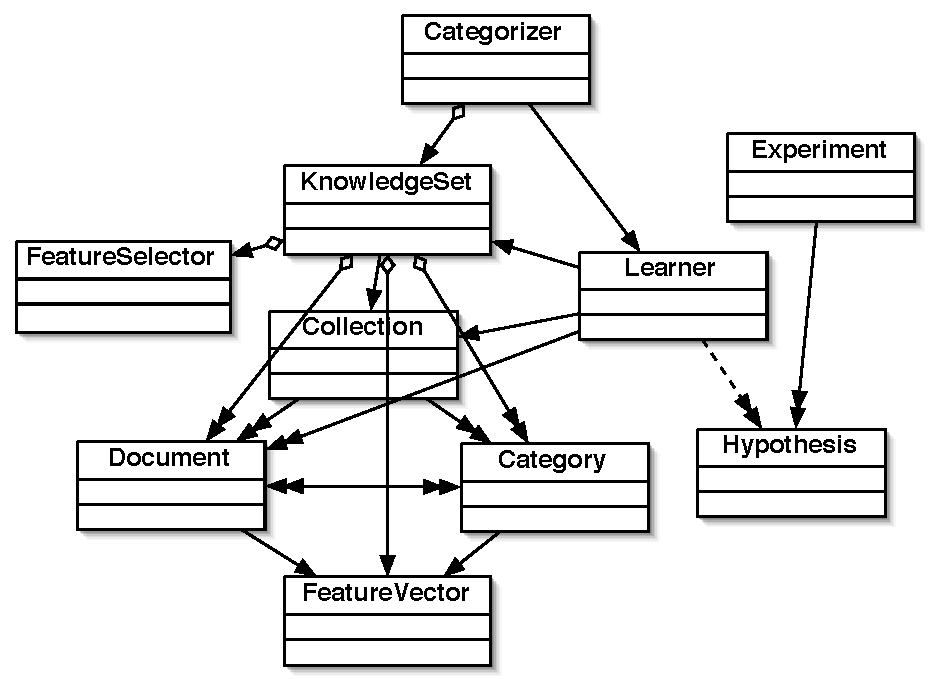
\includegraphics[width=\linewidth]{figures/classes-uml.pdf}
\caption{Class composition diagram for AI::Categorizer}
\label{classes-uml}
\end{figure}

Some examination of the basic relationships between classes and the
responsibilities of each class is helpful before looking at the design
in more detail.  The major classes in the AI::Categorizer framework
are:

\begin{description}

\item[KnowledgeSet]

The KnowledgeSet class represents a set of processed documents, a set
of categories, and a many-to-many mapping between the two sets.
Processing may involve tokenization, stopword removal, linguistic
stemming, feature selection, and vector weighting.  Note that the term
``knowledge set'' is somewhat unique to this project.

A KnowledgeSet contains references to many Document objects and
Category objects.  It uses Collection objects to instantiate Document
and Category objects.  It uses a FeatureSelector object to perform
feature selection.  It also contains a FeatureVector object
representing the features present in all documents.

\item[FeatureSelector]

Feature selection is performed by subclasses of the FeatureSelector
class.  Each KnowledgeSet object contains a FeatureSelector
object--the KnowledgeSet provides the information necessary to do
feature selection, and the FeatureSelector performs the desired
feature selection algorithm.

\item[Collection]

Because data sets in text categorization may be very large, and
because their documents may exist in several different underlying
storage mechanisms (e.g. as files in a filesystem, sections of a
larger XML file, or fields in a database), a Collection class provides
an abstract interface to a set of stored documents, together with a
way to iterate through the set and return Document objects.

A Collection object may be used in several contexts within the
framework.  For instance, a KnowledgeSet instantiates its Document and
Category objects through a Collection object.  A Learner object may
also mass-categorize the Documents in a Collection object.

\item[Document]

Each text document is represented by a Document object, or an object
of one of its subclasses.  Each document class contains methods for
turning a bunch of data into a Feature Vector.  Each document also has
a method to report which categories it belongs to.

\item[Category]

Each category is represented by a Category object.  Its main purpose
is to keep track of which documents belong to it, though it also
contains methods for examining statistical properties of an entire
category.

\item[Learner]

The abstract Learner class can train on a set of pre-categorized
documents and subsequently categorize unseen Document objects.  Its
concrete subclasses implement specific categorization algorithms like
Naive Bayes, SVM, Decision Tree, and so on.

\item[FeatureVector]

Most categorization algorithms don't deal directly with documents'
data, they instead deal with a \emph{vector representation} of a
document's features.  Most often, documents are represented using the
``Bag of Words'' model \cite{XXX}, i.e. a non-ordered, weighted set of
features.  The FeatureVector class provides an interface to the
operations one may perform on these vector representations, such as
querying features' presence or absence in a document, adding vectors
to each other, and so on.

\item[Hypothesis]

The result of asking a Learner to categorize a previously unseen
document is a Hypothesis object.  It may be queried for information
about which categories were assigned, which category was the single
most appropriate category, what scores were assigned to each category,
and so on.

\item[Experiment]

The Experiment class can examine the results of many categorization
decisions (i.e., many Hypothesis objects) and may be queried for
aggregate information about the results.  This is often used in order
to determine the quality (as measured by precision, recall, error,
etc.) of a Learner on a collection of test documents.

\item[AI::Categorizer]

XXX need to write about the umbrella class

\end{description}

\section{Design Patterns in AI::Categorizer}

In order to shed light on the design of the AI::Categorizer framework,
analysis ...


\subsection{Iterator}

The Iterator pattern provides ``a way to access the elements of an
aggregate object sequentially without exposing its underlying
representation.'' \cite[p. 257]{gamma:95} Its main purpose is to
decouple the traversal process on an object's aggregate members from
the object's internal data structure implementation.  In this way,
clients can iterate through aggregate objects without knowing the
objects' internal structure.

In the AI::Categorizer framework, it is often necessary to iterate
through collections of documents and perform some action on them.  For
example, the documents may form a training set for a Learner to base a
model on, or they may form a test set on which to evaluate the model.

The Collection class implements the Iterator pattern
\cite[p. 257]{gamma:95} over documents in the framework.  Figure
\ref{Iterator-collection} shows the main relationships involved in
this pattern.

\begin{figure}
\includegraphics[width=\linewidth]{figures/Iterator.pdf}
\caption{The Iterator pattern in the Collection class}
\label{Iterator-collection}
\end{figure}


\cite[p. 259]{gamma:95} suggests that the most common reasons for
using a formal custom iterator are:

\begin{itemize}

\item to access an aggregate object's contents without exposing its
internal representation.

\item to support multiple traversals of aggregate objects.

\item to provide a uniform interface for traversing different
aggregate structures.

\end{itemize}

The first and third reasons are most germane to the document iteration
process.  As explained in section \ref{Document format}, it is
important that the framework can directly import documents from their
various underlying storage mechanisms in order to prevent unnecessary
duplication of data.  In order to hide the details of the storage
mechanism from the rest of the framework, a Collection object
retrieves documents from several storage mechanisms and returns them
as Document objects.  It provides a unified interface to iteration
over stored documents so that the various classes that need to perform
this iteration (chiefly Learner and KnowledgeSet) don't need to be
aware of storage issues.  In this sense, the ``internal
representation'' of the aggregate structure is often external to the
framework itself, and may be files in a filesystem, entries in a
database, records in an XML document, among others.

In addition to providing a generic interface to a stored collection of
documents, the Iterator pattern allows clients of the Collection class
to use memory efficiently.  A Collection object will typically defer
creation of its Document objects until its client calls its
\texttt{next()} method.  In this way, the Collection doesn't store all
the Documents in memory simultanously--if the client needs to do so,
it can, or it can merely query properties of the Documents and dispose
of them in turn.

In order to decouple the storage mechanism from the internal format of
the document, a Collection class can return many ...


\subsection{Composite}
\begin{figure}
\includegraphics[width=\linewidth]{figures/Composite.pdf}
\caption{The Composite pattern in the Learner::Ensemble class}
\label{Composite-ensemble}
\end{figure}

\subsection{Adapter}
\begin{figure}
\includegraphics[width=\linewidth]{figures/Adapter.pdf}
\caption{The Adapter pattern in the Learner class}
\label{Adapter-learner}
\end{figure}

\subsection{Strategy}
\begin{figure}
\includegraphics[width=\linewidth]{figures/Strategy.pdf}
\caption{The Strategy pattern in the Learner class}
\label{Strategy-learner}
\end{figure}

\begin{figure}
\includegraphics[width=\linewidth]{figures/Strategy-feasel.pdf}
\caption{The Strategy pattern in the FeatureSelector class}
\label{Strategy-feasel}
\end{figure}

\subsection{Factory Method}

\chapter{Implementation}

\section{Language}
\section{Data Structures}

\chapter{Evaluation}

\section{Descriptions of corpora}
During development and testing, several data sets are used for
framework testing and application building.  The main data sets are
listed here.


\subsection{ApteMod (Reuters-21578)}


The "ApteMod" version of the Reuters-21578 corpus has become a
standard benchmark corpus in evaluating Text Categorization systems.
It is a collection of 10,788 documents from the Reuters newswire
service, partitioned into a training set with 7769 documents and a
test set with 3019 documents.  The total size of the corpus is about
17.5 Mb.  It is available from
http://moscow.mt.cs.cmu.edu:8081/reuters\_21578/ in SMART format.


\subsection{SignalG}
This corpus consists of 122,919 financial announcement documents from
the Australian Stock Exchange between January 4 and December 29, 2000.
The documents are hand- categorized according to whether they indicate
"market sensitivity" or not.  Every document is a member of either the
"sensitive" or "insensitive" category--we can view this as two
categories that partition the corpus, or as a single category
"sensitive" that some documents belong to and others don't.  The
documents are split into a training set of 81,814 documents and a test
set of 41,105 documents.


\subsection{DrMath}
This is a smallish collection (26.5 Mb) of English-language messages
sent to the "Ask Dr. Math" question-and-answer service for students
(http://www.mathforum.org/dr.math/).  It consists of messages
containing math questions, categorized by topic and grade level.  Each
category specifies both topic and grade level information (i.e. "High
School Geometry"), so these categorization tasks are not generally
separable into a categorization by topic and a categorization by
level.  The corpus is divided into a training set with 5304 documents
and a test set with 1326 documents.  The corpus is not available for
direct download, but you may contact Ken Williams for details.


\subsection{Reuters-CRC}
This is a collection of financial announcements gathered from the
Reuters financial service in the year 2000.  It represents all
announcements sent by the top 500 companies on the Australian Stock
Exchange (determined by trading volume) during 2000.  There are 27,874
documents, partitioned randomly into 18,568 training documents and
9,306 test documents (105 Mb training, 52.5 Mb test).  We have imposed
a categorization scheme on the data set by examining trends in related
training data, so that each document becomes a member of either the
category "insensitive" or "sensitive", similar to the SignalG data
set.  The corpus is the property of Capital Markets Cooperative
Research Centre and is not available for use by outside groups.


\section{Performance evaluation}

\section{Applications}

\chapter{Conclusion}

\bibliographystyle{plain}
\bibliography{TC-references}

\end{document}
